\documentclass{beamer}

\usepackage{amsmath}
\usepackage{tikz}
\usepackage{ifthen}

\title{Zero-Knowledge Proofs}
\subtitle{Part 1: Knowing More Than Zero}
\author{Isaac Carruthers}

\tikzset{
    pics/my hat graph/.style n args={6}{
        code={
            \node[draw,fill=#1] at (0,0) (a) {A};
            \node[draw,fill=#2] at (0,1) (b) {B};
            \node[draw,fill=#3] at (1,0.5) (c) {C};
            \node[draw,fill=#4] at (2,0) (d) {D};
            \node[draw,fill=#5] at (2,1) (e) {E};
            \node[draw,fill=#6] at (3,1) (f) {F};
            \draw[] (a) -- (b);
            \draw[] (a) -- (c);
            \draw[] (c) -- (b);
            \draw[] (c) -- (e);
            \draw[] (c) -- (d);
            \draw[] (f) -- (e);
        }
    }
}

\begin{document}

\frame{\titlepage}

\frame{\frametitle{What do we Want?}
\begin{itemize}
	\item Paul has some information, and he needs to prove some statement about it to Veronica.
	\item Veronica needs to verify that Paul's statement is true.
	\item Paul does not trust Veronica, and does not want to show her anything beyond
	the fact that his statement is true.
\end{itemize}
}

\frame{\frametitle{What Guarantees do we Need?}
\begin{itemize}
	\item {\bf Completeness:} If the statement is true, then Veronica should
	always be convinced that it is true.
	\item {\bf Soundness:} If the statement is false, there should be no way for Paul
	to convince Veronica.
	\item {\bf Zero-knowledge:} If the statement is true, Veronica learns nothing other
	than the fact that the statement is true. Another way to frame this is that Veronica
	already knows exactly what her interaction with Paul will look like if the statement
	is true.
\end{itemize}
}

\frame{\frametitle{An Example Problem}
\begin{itemize}
	\item I have a big graph, but Google has a big computer.
	\item I want to pay Google to figure out a 3-coloring for my graph.
	\item BUT! We live in a cryptopia, where monetary transactions are instant
	and irrevocable, and trust counts for nothing.
	\item How do I know Google has solved my problem before I give them my money?
\end{itemize}
\vspace{12pt}
\centering
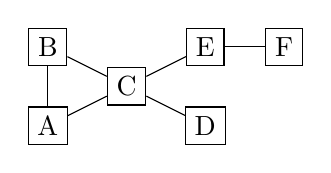
\begin{tikzpicture}
    \draw pic {my hat graph={white}{white}{white}{white}{white}{white}};
\end{tikzpicture}
}

\frame{\frametitle{Beginnings of a Solution}
\begin{enumerate}
	\item I agree on 3 colors with Google.
	\item Google rents out a warehouse, and lays out a colored version of my graph.
	\item Google covers every node with a hat, so I can't see the colors.
	\item I enter the warehouse, and pick an edge.
	\item Google uncovers both nodes connected to the edge, and I check that:
	\begin{enumerate}
		\item both nodes are one of the three agreed-upon colors,
		\item and they are different colors.
	\end{enumerate}
\end{enumerate}
}

\frame{\frametitle{Beginnings of a Solution}
\centering
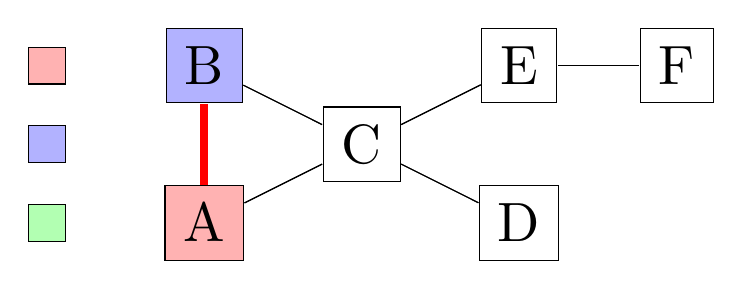
\begin{tikzpicture}[scale=2, every node/.style={scale=2}]
	\node[draw,fill=red!30] at (-1, 1) (x) {};
	\node[draw,fill=blue!30] at (-1, 0.5) (y) {};
	\node[draw,fill=green!30] at (-1, 0) (z) {};
    \draw pic {my hat graph={white}{white}{white}{white}{white}{white}};
	\pause
	\draw[line width=1mm,red] (a) -- (b);
	\pause
    \draw pic {my hat graph={red!30}{blue!30}{white}{white}{white}{white}};
	\draw[line width=1mm,red] (a) -- (b);
\end{tikzpicture}
}

\end{document}
